\documentclass[border=4pt]{standalone}
\usepackage{pgfplots}
\pgfplotsset{compat=1.18}

\begin{document}
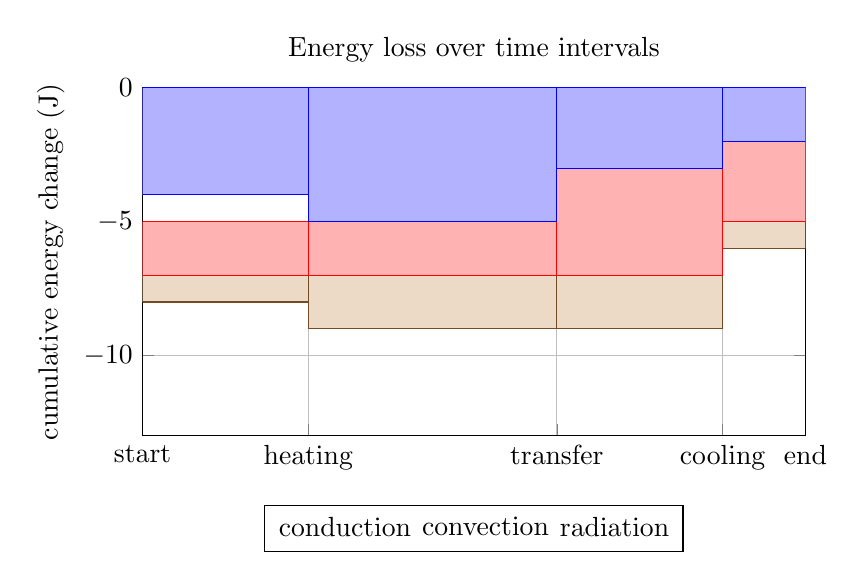
\begin{tikzpicture}
  \begin{axis}[
    ybar interval stacked=minus,
    stack negative=on previous,
    width=10cm,
    height=6cm,
    xmin=0,
    xmax=8,
    ymin=-13,
    ymax=0,
    xtick={0,2,5,7,8},
    xticklabels={start,heating,transfer,cooling,end},
    ylabel={cumulative energy change (J)},
    title={Energy loss over time intervals},
    grid=major,
    legend style={at={(0.5,-0.2)},anchor=north,legend columns=-1}
  ]
    \addplot coordinates {(0,4) (2,5) (5,3) (7,2) (8,0)};
    \addplot coordinates {(0,3) (2,2) (5,4) (7,3) (8,0)};
    \addplot coordinates {(0,1) (2,2) (5,2) (7,1) (8,0)};
    \legend{conduction,convection,radiation}
  \end{axis}
\end{tikzpicture}
\end{document}
